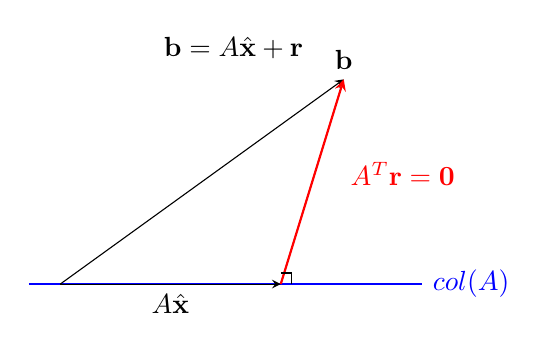
\begin{tikzpicture}[scale=1.0,>=stealth]
% col(A) as horizontal line (1-D), A xhat on it, r vertical
\draw[thick,blue] (-0.4,0) -- (4.6,0) node[right]{$\operatorname{col}(A)$};
\coordinate (O) at (0,0);
\coordinate (p) at (2.8,0);
\coordinate (b) at (3.6,2.6);
\draw[->] (O) -- (p) node[midway,below]{$A\hat{\mathbf x}$};
\draw[->] (O) -- (b) node[above]{$\mathbf b$};
\draw[->,thick,red] (p) -- (b);
\draw (2.8,0.14) -- (2.94,0.14) -- (2.94,0);
\node[red] at (4.35,1.4) {$A^{T}\mathbf r=\mathbf 0$};
\node at (2.2,3.0) {$\mathbf b=A\hat{\mathbf x}+\mathbf r$};
\end{tikzpicture}
